%==================================================================================================
\FloatBarrier
\chapter{Experiments overview}

%--------------------------------------------------------------------------------------------------
\FloatBarrier
\section{Verification of environmeint}
Because in the target implementation of a neural network, the critical element is high 
performance and small size in memory, both for the network model and for the code itself. 
Therefore, it was decided to use the C language because it provides precise control over data 
representation in memory and has minimal memory overhead for the generated code. 
During the initial phase of the experiments, a solution based on combining C with C++ 
will be used. The reason for this approach is the possibility of using design solutions and 
ready-made libraries not available in pure C, which will ensure a much shorter prototyping period.
The downside of this approach is the need to rewrite the final prototype from C ++ to pure C 
before installing it on the target platform. 
However, the experience of the research team so far shows that this approach allows for the 
fastest implementation of the project. 
The problem that resulted from this approach is the lack of direct integration of the created 
solution with the Ai Gym environment used so far, which was written in Python and requires that 
the code using it also be written in this language. 
There are three workarounds for this issue: 
\begin{enumerate}
	\item Use of a dedicated simulation environment for C / C ++.
	\item Integration between the simulation and the neural network employing a library that 
		enables the integration of C functions in Python. 
	\item Implementation of simulations and networks as separate processes together with 
		communication between them based on messages encoded in ASCII.
\end{enumerate}
The first option was immediately rejected due to delays in bringing an entirely new tool 
to the design. 
Several attempts have been made to integrate Python and C ++. This approach turned out to be 
problematic by imposing limitations on possible solutions on the C ++ side. 
An additional drawback was the low portability of the solution and a significant increase in the 
complexity of the compilation environment. 
A solution was chosen based on transferring data between two separate processes using pipes.
\begin{figure}[htb] 
	\label{fig:experiment_pipes}
	\centering
	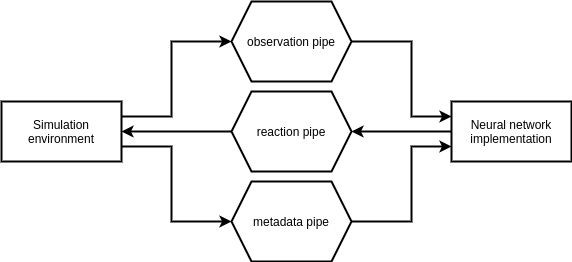
\includegraphics[width=\textwidth]{figures/experiment_pipes}
	\caption{Information flow between simulation an network.}
\end{figure}

As shown in Figure \ref{fig:experiment_pipes}, the system consists of three streams, 
observations, reactions, and metadata. 
Both the observation and reaction pipelines send single vectors separated by a space and terminated
by a line break. 
The data is then converted into the appropriate Python-side Numpy vector and C ++-side Armadillo 
matrix. 
The metadata pipeline, on the other hand, transmits additional information that is not part of 
the observation-reaction loop but is required for the correct interaction between the processes 
and for the training algorithm to be performed.

%--------------------------------------------------------------------------------------------------
\FloatBarrier
\section{Testing basic implementation of NEAT}

%--------------------------------------------------------------------------------------------------
\FloatBarrier
\section{NEAT-23, learing implementation}

%--------------------------------------------------------------------------------------------------
\FloatBarrier
\section{NEAT-23, execution implementation}

%--------------------------------------------------------------------------------------------------
\FloatBarrier
\section{On device}
